\documentclass[a4paper,12pt]{article}
\usepackage[brazilian]{babel}
\usepackage[utf8]{inputenc}
\usepackage[T1]{fontenc}
\usepackage{amsmath}
\usepackage{algorithm}
\usepackage[noend]{algpseudocode}
\usepackage{graphicx}
\usepackage{subfigure}
\usepackage{multirow}
\usepackage{multicol}
\usepackage{verbatim}

\title{Classificação não-supervisionada hierárquica de artigos jornalísticos}
\author{Cirillo Ribeiro Ferreira \\ Orientador: Prof. Dr. Alair Pereira do Lago}
\graphicspath{{images/}}

\begin{document}
\hyphenation{i-ma-gem do-cu-men-tos di-fe-ren-tes m\'a-xi-ma a-pre-sen-ta-dos ou-tros e-li-mi-nar e-xer-c\'i-cios me-lho-ra-ram me-lho-rar ta-ma-nho co-li-ne-a-res e-li-mi-nar sa-li-ên-cias co-mer-ci-ais}
\maketitle
\newpage

\section*{Resumo}
...

\newpage

\tableofcontents
\newpage
\section {Introdução}
A tarefa de classificar e agrupar documentos textuais remonta desde a antiguidade, iniciando-se na criação da primeira biblioteca do mundo em Nínive, Assíria (atual Iraque), por volta do século VII a.C. Desde então, profissões como bibliotecário, documentalista e arquivista foram criadas para atuar na organização desses documentos que vem sendo produzidos pela humanidade.

Porém com a criação da internet e a popularização de seu uso como ferramenta de comunicação, houve uma explosão de informação que tornou praticamente impossível a classificação desses novos tipos de documentos de maneira manual.

A área de classificação de documentos é bem interessante e possui diversas aplicações práticas como classificação de spam, identificação do idioma utilizado e análise de sentimento, porém, em especial, artigos jornalísticos têm um enorme desafio devido à grande quantidade de novos documentos criados diariamente e a diversidade de temas abordados, especialmente em blogs, mas que carecem de melhor organização.

\subsection{Motivação}
\label{sec:motivacao}

A motivação desse trabalho vem da insatisfação com a falta de tempo para uma leitura mais crítica e ciente de um contexto maior devido a enorme quantidade de notícias que estamos sujeitos a receber todos os dias e da organização simplória feita pelos grandes portais de notícias.

O motivo de se utilizar algoritmos não-supervisionados vem da necessidade de encontrar relações implícitas entre os artigos e também da diversidade e quantidade de artigos disponíveis para classificação, uma vez que fica quase que impossível criar manualmente um conjunto de treinamento para subsídio de um algoritmo supervisionado.

Ao contrário da classificação supervisionada, a classificação não-supervisionada não necessita de um conjunto de treinamento como entrada, permitindo o seu uso em conjuntos de dados bem variados, algo que é bem comum em artigos jornalísticos.

A ideia não é separar os artigos jornalísticos em grupos muito generalistas comumente usados em jornais ou portais de notícias, como por exemplo as seções: Brasil, Mundo, Economia e Esportes. Mas sim, encontrar grupos mais intrínsecos que representem com mais acurácia a informação passada por esses artigos …..

[Talvez explicar a diferença entre classificação e agrupamento: Livro sistemas inteligentes, pag 318]

Segundo Martin Ester \textit{et al.} [7], existem alguns desafios da área de agrupamento de documentos como: alta dimensionalidade da coleção, onde cada palavra distinta na coleção constitui uma dimensão, e quanto maior a dimensão, maior o desafio para a construção de um algoritmo escalável e eficiente; grande volume de dados; alta precisão e consistência, dependendo do tipo de documentos, alguns algoritmos apresentam resultados muito abaixo do esperado; e descrição mais significativa dos grupos, pois facilita a utilização pelos usuários.

[Agrupamento é uma das mais antigas atividades mentais humanas, usada para tratar uma quantidade enorme de informações que recebemos todos os dias [1].]

\subsection{Objetivos}

O trabalho de classificação não-supervisionada dos artigos jornalísticos foi dividido em duas partes:

\begin{itemize}
%\item Estudos das principais classes de algoritmos para agrupamento de documentos textuais.
\item Criação de uma biblioteca para agrupamento de artigos jornalísticos.
\item Proposta e implementação do sistema hVINA (\textit{Hierarchical Viewer of News Articles}) para análise de agrupamento de artigos jornalísticos.
\end{itemize}

A representação de um agrupamento de documentos é geralmente feita através de um dendrograma, como na figura \ref{fig:resultado}.

\begin{figure}[h]
    \begin{center}
        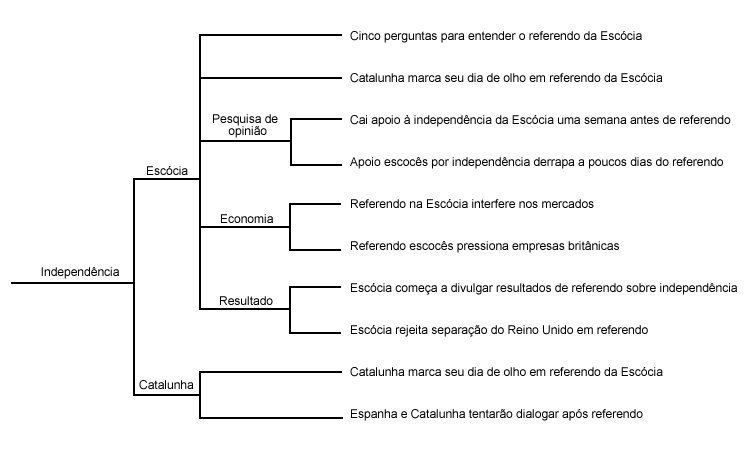
\includegraphics[scale=0.4]{resultado.png}
    \end{center}
    \caption{Esquema do resultado esperado}
    \label{fig:resultado}
\end{figure}

\subsection{Organização do trabalho}

%Na seção \ref{sec:arquitetura} é explicada a arquitetura de um sistema para análise e leitura de tablóides que seja robusto e expansível a vários tipos de tablóides. A seção \ref{sec:segmentacao} descreve a etapa de segmentação de uma página de um tablóide. A seção \ref{sec:detect_ocr} descreve a etapa de detecção de textos e uso de um programa de OCR. Na seção \ref{sec:resultados} são apresentados os resultados obtidos e na seção \ref{sec:conclusoes} são explicitadas as conclusões finais do trabalho, assim como uma avaliação do cumprimento dos objetivos propostos. Na seção \ref{sec:subj} é apresentada uma análise subjetiva do curso do Bacharelado em Ciência da Computação.

No capítulo 2 é apresentado os fundamentos da área de reconhecimento de padrão e mais especificamente de análise de agrupamento. No capítulo 3 é discutido em detalhe o algoritmo FIHC, escolhido para ser implementado na biblioteca e sistema propostos no 4o capítulo para o agrupamento de artigos jornalísticos. No capítulo 5 é feito a avaliação do sistema na coleção de artigos do jornalista José de Paiva Netto e também da coleção da Reuters. E por fim, no capítulo 6 são apresentadas as conclusões desse trabalho.

\newpage
\section {Fundamentos}
\label {sec:fundamentos}
Antes de apresentar e discutir sobre a biblioteca desenvolvida e o sistema proposto, será apresentado alguns conceitos básicos necessários para a compreensão do conteúdo e dos resultados obtidos.

\subsection{Reconhecimento de padrão}
\label{sec:reconhecimento_padrao}

Segundo Theodoridis e Koutroumbas  [1], reconhecimento de padrão é uma área da ciência cujo objetivo é a classificação de objetos dentro de um número de categorias ou classes. Esses objetos de estudo variam de acordo com cada aplicação, podem ser imagens, sinais em forma de ondas (como voz, luz, rádio) ou qualquer tipo de medida que necessite ser classificada. As implicações práticas desses estudos permeiam todas as áreas de atuação humana, principalmente numa sociedade pós-industrial, onde a necessidade de automação das diversas atividades é essencial.  Sua aplicação vai desde sistemas que utilizam visão computacional, passando por reconhecimento de caracteres até sistemas para auxílio à domada de decisão.

\subsubsection{Formas de processo de aprendizagem}
\label{sec:formas_processo_aprendizagem}

Na área de reconhecimento de padrão os algoritmos utilizam técnicas de aprendizagem computacional para a realização de alguma tarefa e eles são geralmente classificados de acordo a necessidade de intervenção humana durante alguma fase de aprendizagem do algoritmo. São elas: aprendizagem supervisionada,  aprendizagem não-supervisionada e aprendizagem semi-supervisionada.

A classificação supervisionada consiste na utilização de um conjunto de dados previamente classificados (ou anotados), que servirá na construção de um modelo para a classificação de novos objetos. Ou seja, algoritmos que utilizam esse conjunto de dados fazem uso de um conhecimento a priori, originado de uma fonte externa. Esse conjunto de dados inicial é denominado de conjunto de treinamento (\textit{training set}). Porém, em muitos casos a criação de um conjunto de treinamento é inviável devido à natureza do problema [pegar exemplos: não se conhece previamente todas as classes]. Para esses tipos, é então empregado a classificação não-supervisionada, que não faz uso de um conjunto de treinamento, pois o próprio algoritmo busca descobrir similaridades intrínsecas nos objetos e agrupa aqueles objetos mais similares. [1, 2, 3]

Por fim, a classificação semi-supervisiona emprega técnicas da classificação supervisionada e não-supervisionada, geralmente com um conjunto pequeno de treinamento.

No contexto de reconhecimento de padrão, é comum chamar a classificação supervisionada de apenas classificação e a classificação não-supervisionada de análise de agrupamento, ou simplesmente agrupamento (do inglês \textit{clustering}). A figura ? mostra o esquema das formas de aprendizagem.

[Seria muito bom se colocasse um esquema dessas formas de processo de aprendizagem]

\subsection{Análise de agrupamento}
\label{sec:analise_agrupamento}

Análise de agrupamento é uma classificação de padrão que emprega o processo de aprendizagem não-supervisionada e tem como objetivo o particionamento de objetos em grupos cujo membros sejam similares entre si e diferentes dos membros de outros grupos [2]. Porém, também tem os objetivos secundários de evitar grupos muito pequenos ou muito grandes e encontrar grupos que façam sentido ao usuário. Segundo Theodoridis e Koutroumbas [1], a análise de agrupamento é largamente utilizada na resolução de diversos problemas, e pode ser encontrada em outras áreas por nomenclaturas diferentes, como taxonomia numérica em biologia, e tipologia na área das ciências sociais.

Um grande problema enfrentado na análise de agrupamento é a dimensionalidade ou variáveis dos dados envolvidos, sejam eles observações de estrelas no céu, observações de organismos vivos na natureza ou documentos textuais disponíveis na internet, e uma técnica bastante utiliza para tentar solucionar tal problema é a redução dimensional através da extração de características, que envolve em sintetizar os dados em características mais relevantes para o problema principal sem perda de informação.

\subsection{Agrupamento de documentos textuais}
\label{sec:agrupamento_doc_textual}

Uma aplicação da análise de agrupamento é na organização de documentos. Geralmente ao fazer alguma consulta em sistemas de busca são retornadas centenas de documentos que possuem algum tipo de relevância à consulta, porém esse grande número de resultado pode inviabilizar a utilização desses sistemas, por isso a maioria deles utiliza algumas técnicas de análise de agrupamento para organizar automaticamente os resultados em categorias que fazem sentido ao usuário. 

Em especial, quando se fala em documentos textuais, o processo de redução dimensional através de extração de características dos dados é de sensível importância devido à grande redundância dos dados, que neste caso, são sentenças ou palavras. Processar os documentos sem antes usar uma boa técnica de redução dimensional acarreta quase sempre em baixa eficiência da solução.

\subsection{Tipos de algoritmo de agrupamento}
\label{sec:tipos_algoritmo_agrupamento}

Um algoritmo de agrupamento objetiva encontrar as classes naturais das observações, baseados em alguma similaridade. Existem diversos algoritmos para agrupamento desenvolvidos [1, 2], porém neste capítulo serão citadas duas categorias de algoritmos mais empregados nesse processo. Uma explicação com aspectos mais detalhados desses métodos pode ser encontrada em [1, 2].

\subsubsection{Agrupamento plano}
\label{sec:agrupamento_plano}

Agrupamento plano é a categoria de algoritmos cujo os grupos resultantes são dados num único nível, onde nenhum grupo tem relação com outro. O principal algoritmo dessa categoria é o \textit{k-means} [3].

Antes de falar do \textit{k-means} é preciso relembrar um ponto essencial ao entendimento desse algoritmo, que é a definição de centroide. Na geometria, o centroide é o ponto central de uma figura. Dessa forma, dado um grupo, se ligarmos com um segmento de linha as observações mais distantes podemos visualizar uma figura geométrica, e o centroide desse grupo seria a observação mais próxima ao centro dessa figura.

[Inserir algoritmo k-means]

Em termos gerais, o objetivo do \textit{k-means} é dividir n observações em \textit{k} grupos, minimizando a média das distâncias euclidianas quadráticas entre as observações e os respectivos centroides dos grupos, ou seja, cada observação é associada ao grupo cujo o centroide está mais próximo. 

O algoritmo inicia com uma escolha aleatória dos \textit{k} centroides e a cada iteração é feito um refinamento na escolha desses centroides até que não haja mais reescolha dos centroides ou até que se atinja um número predefinido de iterações. A figura \ref{fig:passos_kmeans} exemplifica a sequência descrita acima.

Há duas propriedades importantes do \textit{k-means}:

\begin{itemize}
\item Cada objeto deve pertencer ao menos um dos \textit{k} grupos.
\item Nenhum objeto pertence a mais que um grupo.
\end{itemize}

\begin{figure}[h]
    \begin{center}
        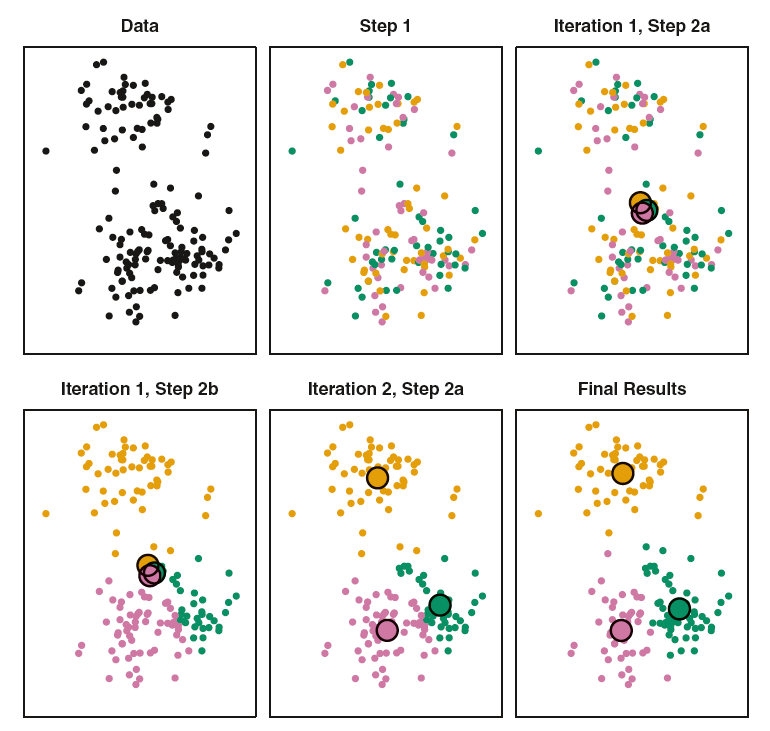
\includegraphics[scale=0.5]{k_means_algorithm.png}
    \end{center}
    \caption{Sequência de passos do algoritmo k-means, retirado de [13]}
    \label{fig:passos_kmeans}
\end{figure}

Um cuidado especial na utilização desse algoritmo é na escolha do número de grupos desejado. Uma escolha inadequada poderá resultar em um mau agrupamento, unindo duas classes naturais em um único grupo ou dividindo uma classe natural em dois grupos,  [falar do fato de não ser deterministico] porém algumas técnicas tem sido desenvolvidas para resolver esse problema [2, 3, ?]. (colocar mais referências a artigos para solução desse problema) Um exemplo de problema que pode ocorrer está ilustrado pela figura \ref{fig:problema_kmeans}.

\begin{figure}[h]
    \begin{center}
        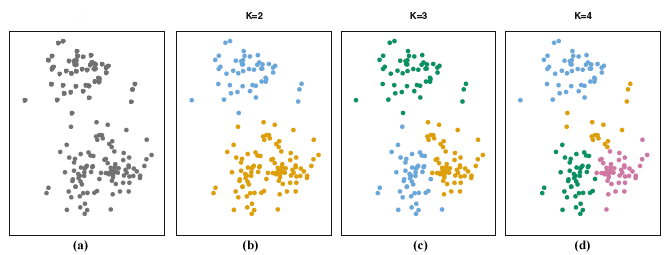
\includegraphics[scale=0.8]{cluster_1.png}
    \end{center}
    \caption{Em (a) é mostrado um conjunto de dados fictício com três classes naturais. Em (b) quanto é escolhido o número de grupos k = 2, as classes naturais 2 e 3 são unidas num único grupo. Em (c), com k = 3, os grupos refletem as classes naturais dos dados, e em (d) com k = 4 a classe natural 3 é dividida entre dois grupos.}
    \label{fig:problema_kmeans}
\end{figure}

Conforme John Wang [9], o algoritmo \textit{k-means} não é adequado para descobrir grupos de tamanhos que variam muito, um cenário comum em agrupamento de documentos. Além disso, é sensível a ruídos que pode ter uma grande influência sobre a escolha do centroide de um grupo, que por sua vez diminui a precisão do agrupamento. Todavia algoritmos como o \textit{k-medoids} [9] foram propostos para resolver o problema do ruído.

\subsubsection{Agrupamento hierárquico}
\label{sec:agrupamento_hierarquico}

Agrupamento plano geralmente é mais simples e fácil de implementar, porém existem certos tipos de problemas em que a visualização de um agrupamento de um único plano não é suficientemente útil, além disso, como visto no tópico anterior, esse tipo de agrupamento tem dois problemas que são a escolha do número de grupo na entrada e o fato de não serem determinísticos [3]. Dessa forma, algoritmos que criassem agrupamentos com vários níveis e que tivessem como requisito opcional a entrada do número de grupos foram desenvolvidos. Esses algoritmos criam uma árvore hierárquica de grupos, uma estrutura que gera mais informação, uma vez que as relações implícitas entre os grupos ficam mais evidentes.

Existem duas abordagens no funcionamento de um algoritmo hierárquico que são:

\begin{itemize}
\item Abordagem aglomerativa:. Gera a árvore de grupo ao continuamente calcular a similaridade de todos os pares de grupos e unificar o par mais similar (segundo um critério de similaridade), criando a árvore das folhas até a raiz, por isso é também conhecida como abordagem bottom-up. Um exemplo dessa abordagem é ilustrado na figura \ref{fig:hierarchical_algorithm}.

\item Abordagem divisiva: Gera a árvore de grupo da raiz às folhas (top-down), utilizando em cada nível da árvore um algoritmo de agrupamento plano para a divisão dos grupos em nós filhos.
\end{itemize}

\begin{figure}[h]
    \begin{center}
        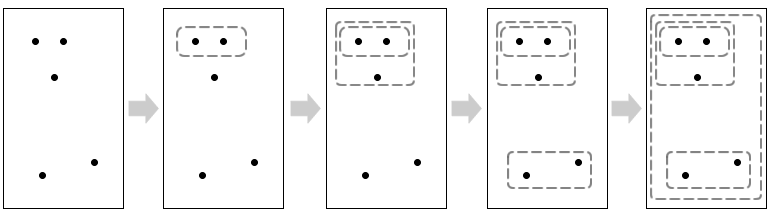
\includegraphics[scale=0.5]{hierarchical_algorithm.png}
    \end{center}
    \caption{Exemplo de um algoritmo hierárquico aglomerativo, retirado de [8], onde o critério de similaridade utilizado é a distância euclidiana.}
    \label{fig:hierarchical_algorithm}
\end{figure}

\subsection{Critério de avaliação}
\label{sec:criterio_avaliação}

Existem 2 tipos de erros que podem ocorrer no processo de agrupamento. O primeiro, chamado de falso positivo (FP) ou erro tipo I, ocorre quando o algoritmo associa dois documentos não similares a um mesmo grupo, e o segundo, chamado de falso negativo (FN) ou erro tipo II, ocorre quando o algoritmo associa dois documentos similares a grupos distintos. Um critério de avaliação justo tem de levar em conta as ocorrências desses dois erros. A tabela ? a seguir, mostra a matriz de contingência entre os documentos e grupos.

[Inserir tabela de contigencia]

Duas medidas importantes na área de reconhecimento de padrão e também na estatística, são a precisão e cobertura do resultado observado. O primeiro, no contexto de reconhecimento de padrão, mede a fração de documentos que estão classificados corretamente no grupo e é dado pela seguinte fórmula:

\begin{equation} P = \frac{TP} {TP + FP} \end{equation}

Já a cobertura mede a fração de documentos que foram classificados corretamente dentre os documentos similares e é dado pela fórmula:

\begin{equation} R = \frac{TP} {TP + FN} \end{equation}

Por exemplo, dado o conjunto de documentos \{1, 2, 3, 4, 5, 6\}, onde $N_{1}$ = \{1, 3, 5\} fazem parte de uma classe natural, ou seja, são similares; e $N_{2}$ = \{2, 4, 6\} fazem parte de outra classe natural. Dado um grupo C = \{1, 3, 4, 5\} a precisão de C em relação a $N_{1}$ é P = 3/4 e a cobertura é R = 3/3 = 1, ou seja, nem todos os documentos de C são similares entre si, apesar de que todos os documentos de $N_{1}$ foram agrupados corretamente em C.

Porém, a utilização de duas medidas para avaliação e comparação de algoritmos torna difícil determinar se um algoritmo é superior a outro ou não. Pois é melhor um algoritmo com alta precisão e baixa cobertura, ou vice-versa? A resposta para essa pergunta depende do contexto onde é aplicado o agrupamento. Segundo Manning et al, na maioria das vezes é mais aceitável o erro de tipo I, pois separar documentos similares em grupos distintos é geralmente pior do que juntar documentos não similares num mesmo grupo [7].

Dado isto, um critério para avaliação bastante utilizado é a medida F (\textit{F-measure}), pois avalia o agrupamento utilizando a média harmônica ponderada da precisão e da cobertura. A medida F é dada por:

\begin{equation} F_{\beta} = (1 + \beta^2) \times \frac{P \times R} {\beta^2 P + R} \end{equation}
onde $\beta^2$ $\in$ [0, $\infty$].

Um valor para $\beta$ bastante utilizado é $\beta$ = 1, pois tanto a precisão quanto a cobertura terão o mesmo peso na medida. Neste caso, a medida seria simplificada da seguinte forma:

\begin{equation} F_{1} = 2 \times \frac{P \times R} {P + R} \end{equation}

Já definindo $\beta$ > 1, a precisão será mais enfatizada em relação à cobertura. Note que para a medida F, o algoritmo não basta ter apenas boa precisão ou apenas boa cobertura, mas sim ambas características, o que a torna um dos critérios mais utilizados para a análise. Porém, ela não é o único critério de avaliação existente. Dentro da área de estudo sobre avaliação de agrupamentos existem critérios internos e externos e a medida F se enquadra na segunda categoria, pois avalia o agrupamento a partir de uma classificação de referência [7].

\newpage
\section {FIHC}
\label {sec:fihc}

\textit{Frequent Itemset-based Hierarchical Clustering} (FIHC) é um algoritmo para agrupamento hierárquico de documentos proposto por Martin Ester \textit{et al.} [7] e que utiliza o conceito de conjuntos de itens frequentes (do inglês \textit{frequent itemset}).

Segundo Martin Ester \textit{et al.}, a ideia utilizada para o critério de agrupamento dos documentos é que existe algum conjunto de itens frequentes para cada grupo (tópico) no conjunto de documentos, e diferentes grupos compartilham poucos conjuntos de itens frequentes.

Segundo os autores, o algoritmo tenta resolver alguns desafios da área como: alta dimensionalidade da coleção, onde cada palavra distinta na coleção constitui uma dimensão, e quanto maior a dimensão, maior o desafio para a construção de um algoritmo escalável e eficiente; grande volume de dados; alta precisão e consistência, dependendo do tipo de documentos, alguns algoritmos apresentam resultados muito abaixo do esperado; e descrição mais significativa dos grupos, pois facilita a utilização pelos usuários.

Um ponto de interesse é que, diferentemente dos algoritmos mais comuns para agrupamento hierárquico, no FIHC a parametrização do número de grupos desejado é opcional, assim o usuário não precisa ter nenhum conhecimento prévio da coleção de documentos.

O algoritmo utiliza a abordagem aglomerativa, descrita na seção 2.4.2, porém ao invés de construir a árvore baseando-se na similaridade entre as observações (documentos) ele a faz baseando-se nos grupos [7]. Possui dois passos principais, que é a construção dos grupos e posteriormente a criação da árvore hierárquica, entretanto antes de apresentá-los é necessário introduzir algumas definições.

\subsection {O que é conjunto de itens frequentes}
\label {sec:conjunto_itens_frequentes}

Por definição, conjunto de itens é o conjunto de palavras que ocorrem em conjunto na coleção de documentos. Logo conjunto de itens frequentes é o conjunto de palavras que ocorrem numa quantidade de documentos acima de um limiar de suporte definido. 

Em outras palavras, assumindo que \emph{l} é o limiar de suporte. Se F é um conjunto de palavras, o apoio (\textit{support} em inglês) de F é a proporção de documentos no qual F é um subconjunto das palavras desses documentos. Assim, dizemos que F é um conjunto de itens frequentes se o seu valor de apoio é \emph{l} ou superior. A tabela \ref{table:colecao_artigos} ilustra um exemplo:

\begin{table}[h]
\centering
\begin{tabular}{ | l | p{10cm} | }
\hline
Documento & Palavras (itens)                                                                   \\ \hline
doc.1     & \{Bolsa, europeia, opera, em, queda, após, anúncio, de, pacote, grego\}            \\ \hline
doc.2     & \{Japão, e, Grécia, ficam, no, 0, a, 0, no terceiro, dia, de, competição\}         \\ \hline
doc.3     & \{Descoberta, de, tumba, misteriosa, anima, Grécia, em, meio, à, crise, europeia\} \\ \hline
doc.4     & \{Grécia, assume, presidência, da, União, Europeia, por, seis, meses\}             \\ \hline
doc.5     &  \{Crise, está, prejudicando, saúde, mental, dos, gregos\} \\
\hline
\end{tabular}
\caption{Coleção de artigos}
\label{table:colecao_artigos}
\end{table}

No exemplo acima, a palavra “Grécia” aparece nos documentos, (2), (3) e (4), assim seu suporte é 3; a palavra “crise” aparece em (3) e (5), logo seu suporte é 2; a palavra “de” ocorre em todos os documentos, exceto em (4) e (5), assim seu suporte é 3; a palavra “europeia” ocorre em (1), (3) e (4), logo seu suporte é 3. Todas as outras palavras ocorrem apenas em um único documento. Logo se for definido o limiar de suporte \emph{l} = 2, teremos como conjuntos de itens frequentes os conjuntos \{Grécia\}, \{crise\}, \{de\} e \{europeia\}. Além disso, as duplas \{Grécia, europeia\}, \{Grécia, de\} e \{europeia, de\} ocorrem em 2 documentos, logo também são conjuntos de itens frequentes.

No caso do algoritmo FIHC, conjuntos de itens frequentes são também denominados de conjuntos globais de itens frequentes, e suporte é denominado de \textit{global support}.

\subsubsection {Algoritmo Apriori}
\label {sec:algoritmo_apriori}

A extração dos conjuntos de itens frequentes é uma das técnicas mais utilizadas para caracterização de dados com objetivo de resumir os atributos gerais mais relevantes de um conjunto de dados. O exemplo mostrado na seção anterior é uma forma de encontrar os conjuntos de itens frequentes, porém esse método não é eficiente quando é utilizado em uma coleção grande de documentos. Um dos algoritmos mais populares para tal propósito, seja em um banco de dados ou em documentos textuais, é o algoritmo Apriori. (wikipedia?)

A algoritmo utiliza a propriedade de anti-monotonicidade [10], onde se um conjunto de itens não é frequente, então todos os seus superconjuntos também não serão.

Ele inicia a busca a partir de uma coleção de conjunto de itens frequentes com cardinalidade k = 1, chamado de $F_{1}$ . A partir daí todos os conjuntos de cardinalidades maiores são obtidos a partir de uma coleção de candidatos C. O algoritmo para quando não encontrar mais nenhum conjunto de itens frequentes. A figura ? mostra o algoritmo:

\begin{algorithm}
\caption{Algoritmo Apriori para extração de conjuntos de itens frequentes em documentos textuais}
\label{algorithm_apriori}
\begin{algorithmic}[1]
\State $F_{1} \gets (\text{Conjunto de itens frequentes de cardinalidade 1})$
\State $k \gets 1$

\While {$F_{k} \neq \emptyset$}
	\State $C_{k+1} \gets candidate\_gen(F_{k}) $
	
	\ForAll {documento d na coleção}
		\State $C'_{d} \gets subset(C_{k+1},d)$
		
		\ForAll {candidato c $\in$ $C'_{d}$}
			\State $c.count \gets c.count + 1$
		\EndFor
		
	\EndFor
	
	\State $F_{k+1} \gets \{ c \in C_{k+1} | c.count \geq \text{suporte mínimo} \}$
	
	\State $k \gets k + 1$
\EndWhile

\Return $\cup_{k} F_{k}$
\end{algorithmic}
\end{algorithm}

\subsection {O que é \textit{cluster frequent item} e \textit{cluster support}}
\label {sec:cluster_frequent_item_e_cluster_support}

Dado o grupo $C_{i}$, um elemento de um conjunto global de itens frequentes é denominado de \textit{cluster frequent item} de $C_{i}$ se este elemento está contido em um número mínimo de documentos de $C_{i}$, definido como \textit{minimum cluster support}.

Além disso, \textit{cluster support} de um item em $C_{i}$ é definido como a porcentagem de documentos de $C_{i}$ que contém o item.

\subsection {O que é tf-idf}
\label {sec:tf_idf}

Tf-idf é uma medida estatística usada para avaliar o quão importante uma palavra é para um documento em relação a uma coleção de documentos. (wikipedia)  A ideia é que se uma palavra é tão comum em diferentes documentos da coleção, então provavelmente ela tem pouca relevância, por exemplo, a conjunção aditiva “e”. A importância aumenta proporcionalmente ao número de vezes que uma palavra aparece no documento, mas é compensado pela frequência da palavra no corpus. O tf-idf é dado pelo produto de duas medidas: a frequência do termo e a frequência inversa do documento, dado por:

\begin{equation} tf-idf(t, d) = tf(t, d) \times \log \frac{N} {df(t)} \end{equation}
onde $tf(t,d)$ é a razão entre o número de vezes que o termo $t$ aparece no documento $d$ e a quantidade de termos em $d$; $N$ é a quantidade de documentos na coleção e $df(t)$ é a quantidade de documentos da coleção que possui o termo $t$. Existem diversas variantes dessa medida como visto em [3].

\subsection {Construção dos grupos}
\label {sec:construcao_grupos}

Apresentado alguns conceitos relacionados ao FIHC, vamos ao algoritmo propriamente dito. Como já dito, o primeiro passo do algoritmo é construir os grupos, e isso é feito em duas etapas. Primeiramente, os grupos iniciais são construídos a partir dos conjuntos globais de itens frequentes extraídos da coleção e então é feito o processo de disjunção desses grupos para que no final um documento pertença somente a um único grupo.

Na criação dos grupos iniciais, para cada conjunto global de itens frequentes é criado um grupo que inicialmente incluirá todos os documentos que contêm o conjunto de itens em seu corpo. Logo cada grupo possuirá um conjunto de itens frequentes gerador. 

Note que esses grupos podem não ser disjuntos, pois um documento pode conter vários conjuntos de itens frequentes.

[Inserir tabela 1]

[Inserir tabela 2]

\subsubsection {Disjunção dos grupos sobrepostos}
\label {sec:disjuncao_grupos_sobrepostos}

A disjunção é um processo importante, pois garante que ao final do algoritmo cada documento pertença somente ao grupo que melhor o descreva. Para cada documento D, é listado todos os grupos no qual ele pertence, e após isso é calculado para cada um desses grupo C uma medida que indicará a “relevância” de D em relação a C. Essa medida tem o nome de Score e é proposto em [7].

Após os cálculos da medida Score de D para cada grupo C, é mantido o documento somente no grupo que maximizou essa medida. Esse cálculo de relevância de um grupo inicial $C_{i}$ para um documento $D_{j}$ é definido por:

\begin{equation}
\begin{split}
  Score(C_{i} \gets D_{j}) = |\sum_{x}tf-idf(x, D_{j}) * cluster\_support(x)| \\
  - |\sum_{x'}tf-idf(x', D_{j}) * global\_support(x')|
\end{split}
\end{equation}
onde $x$ representa um \textit{global frequent item} que está contido em $D_{j}$ e também é um \textit{cluster frequent item} de $C_{i}$; $x’$ representa um \textit{global frequent item} que está contido em $D_{j}$, mas que não é um \textit{cluster frequent item} de $C_{i}$; $tf-idf(x, D_{j})$ e $tf-idf(x’, D_{j})$ são as medidas tf-idf dos itens $x$ e $x’$ em $D_{j}$; $cluster\_support(x)$ é o \textit{cluster support} de $x$ e $global\_support(x’)$ é o \textit{global support} de $x’$.

[Inserir tabela 3]

O primeiro termo da função $Score(C_{i} \gets D_{j})$ recompensa $C_{i}$ se o \textit{global frequent item} $x$ em $D_{j}$ é também um \textit{cluster frequent item} de $C_{i}$ e o segundo termo penaliza $C_{i}$ se o \textit{global frequent item} $x’$ em $D_{j}$ não é um \textit{cluster frequent item} de $C_{i}$. De acordo com Martin Ester \textit{et al.} [7], intuitivamente, um grupo $C_{i}$ é “bom” para um documento $D_{j}$ se há muitos \textit{global frequent items} em $D_{j}$ que aparecem em “muitos” documentos em $C_{i}$. Se há mais de um grupo que maximiza a medida $Score(C_{i} \gets D_{j})$, então é escolhido o grupo com maior número de itens em seu conjunto de itens frequentes gerador.

Seguindo o exemplo da tabela ?, note que o documento artigo.3 pertence aos grupos C(mercado), C(crise), C(Grécia) e C(mercado, crise). Para se decidir em qual desses grupos o artigo deve permanecer, são calculados os seguintes $Score$:

$Score(C(mercado) \gets artigo.3) = 1 * 1 + 4 * 0,5 + 3 * 0,75 = 5,25$

$Score(C(crise) \gets artigo.3) = 1 * 0,5 + 4 * 1 - 3 * 0,3 = 3,6$

$Score(C(Grécia) \gets artigo.3) = 1 * 1 + 3 * 1 - 4 * 0,4 = 2,4$

$Score(C(mercado, Grécia) \gets artigo.3) = 1 * 1 + 3 * 1 - 4 * 0,4 = 2,4$

Logo, o documento artigo.3 seria mantido apenas no grupo C(mercado).

[Inserir tabela 4]

\subsection {Criação da árvore de grupos}
\label {sec:criacao_arvore_grupos}

Uma vez computado os grupos iniciais, podemos visualizar cada um deles como um tópico ou subtópico na coleção de documentos. Agora é necessário criar a árvore, colocando os tópicos mais generalistas no topo e os mais específicos abaixo. Essa árvore tem como objetivos cria uma estrutura para a navegação entre os documentos e também facilitar a poda dos grupos muito específicos.

Os grupos são inicialmente aninhados na árvore de acordo com a quantidade de itens em seu conjunto global gerador. Dessa forma, aqueles que possuem somente um item, estão no primeiro nível da árvore, e assim por diante. A raiz (nível 0) da árvore é por definição um grupo vazio e sem nenhum item em seu conjunto global de itens frequentes. Como dito no início desse capítulo, o FIHC utiliza a abordagem aglomerativa para a criação da hierarquia, ou seja, para cada grupo C no nível \emph{k} é escolhido um pai dentre os potenciais grupos do nível \emph{k-1}, cujo o conjunto global seja subconjunto dos conjuntos globais de itens frequentes de C. Se houver mais de um potencial pai no nível \emph{k-1}, então é escolhido aquele grupo que maximiza uma medida de ???, similar ao processo descrito na seção 3.4.1. Isso é melhor detalhado em [7].

Uma vez escolhido um grupo pai para cada grupo da coleção, é necessário verificar se é possível unificar os grupos similares ou com tópicos muito específicos, garantindo uma hierarquia mais natural para a navegação e melhorando a acurácia do algoritmo. Isso é feito de duas formas: 1) através do processo de poda dos grupos filhos e 2) unificação dos grupos similares do nível 1.

A medida de similaridade utilizada no algoritmo FIHC utiliza a ideia de tratar um grupo como um documento conceitual, definindo a partir da combinação de todos os documentos do grupo, e a partir daí é tirado a medida através de um cálculo bem similar à medida $Score$ apresentada na seção anterior. Dado um grupo $C_{a}$ e $C_{b}$, a medida de similaridade entre os grupos é calculado a partir da média geométrica entre a similaridade de $C_{a}$ para $C_{b}$ e da similaridade de $C_{b}$ para $C_{a}$. Da seguinte forma:

\begin{equation}
  Inter\_Sim(C_{a} \leftrightarrow C_{b}) = [Sim(C_{a} \gets C_{b}) * Sim(C_{b} \gets C_{a})]^\frac{1} {2}
\end{equation}
onde a similaridade $Sim$ de $C_{a}$ para $C_{b}$ é dado como:

\begin{equation}
  Sim(C_{a} \gets C_{b}) = \frac{ Score(C_{a} \gets doc(C_{b})) }{ \sum_{x}tf-idf(x,doc(C_{b})) + \sum_{x'}tf-idf(x',doc(C_{b})) } + 1
\end{equation}

Em $Sim(C_{i} \gets C_{j})$, a medida $Score$ é a mesma discutida na seção anterior, porém a única diferença é que o documento $doc(C_{j})$ utilizado no cálculo é um documento conceitual, construído a partir da combinação de todos os documentos da subárvore de $C_{j}$, e $tf-idf(x, doc(C_{b}))$ e $tfidf(x’, doc(C_{b}))$ são, respectivamente, as medidas tf-idf dos itens $x$ e $x’$ em $doc(C_{j})$.

\subsection {Rotulagem do grupo}
\label {sec:rotulagem_grupo}

Uma etapa importante no processo de agrupamento é a de rotulagem dos grupos, pois para um usuário entenda o resultado do algoritmo e o utilize sem dificuldades é necessário que a rotulagem seja legível e faça sentido a ele. 

No caso do FIHC, a própria abordagem de criação dos grupos a partir dos conjuntos globais de itens frequentes da coleção e posterior escolha dos \textit{cluster frequent items} torna natural pensar que esses conjuntos de palavras também são bons candidatos para dar nome aos próprios grupos. 

[Exemplo]

\newpage

\begin{thebibliography}{9}
\bibitem{Ma e Zhang03}
    Y. Ma, H. Zhang.
    \emph{Contrast-based image attention analysis by using fuzzy growing}.
    Proceedings of the Eleventh ACM international Conference on Multimedia
    Berkeley, CA, USA.
    2003.

\bibitem{Itti e Koch03}
    L. Itti, C. Koch.
    \emph{A saliency-based search mechanism for overt and covert shifts of visual attention}
    Vision Research, Volume 40, Issues 10-12, Pages 1489-1506,
    ISSN 0042-6989, DOI: 10.1016/S0042-6989(99)00163-7.
    2000.

\bibitem{Liu.et.al07}
    H. Liu, S. Jiang, Q. Huang, C. Xu, W. Gao
    \emph{Region-based visual attention analysis with its application in image browsing on small displays}.
    In Proceedings of the 15th international Conference on Multimedia  (Augsburg, Germany, September 25 - 29, 2007).
    2007.

\bibitem{survey10}
    S. Frintrop, E. Rome, H. I. Christensen.
    \emph{Computational visual attention systems and their cognitive foundations: A survey}.
    ACM Trans. Appl. Percept. 7, 1 (Jan. 2010), 1-39.
    2010.

\bibitem{breuel03}
    T. M. Breuel.
    \emph{High performance document layout analysis}.
    [Online]. Available: http://citeseerx.ist.psu.edu/viewdoc/summary?doi=10.1.1.13.1303
    2003

\bibitem{GOF}
    E. Gamma, R. Helm, R. Johnson, J. Vlissides.
    \emph{Design Patterns: Elements of Reusable Objected-Oriented Software}.
    Addison-Weskey Professional; 1 edition,
    November 10th, 1994

\bibitem{morfologia}
    E.R. Dougherty, R.A. Lotufo.
    \emph{Hands-on Morphological Image Processing}.
    SPIE press,
    2003

\bibitem{tesseract}
    \emph{Tesseract OCR}
    http://code.google.com/p/tesseract-ocr/

\bibitem{duda}
    R. O. Duda, P. E. Hart, D. Stork.
    \emph{Pattern Classification}.
    Wiley-Interscience; 2nd edition,
    October 2000.

\end{thebibliography}
\end{document}
​
